\chapter{Zorro Case Studies}
\label{ch:evaluation}
Test-driven development is a low-level software process that consists of
many short-duration activites---file edit, compilation, unit test, debug, so
on and so forth. Zorro software system collects and analyzes on these
low-level and short-duration activites to detect the existance of
test-driven development with software development stream technology and
rule-based system supports. The test run and pilot study have demonstrated
that Zorro recognized test-driven development successfully. Yet,
following three issues are remained to be resolved before we deploy Zorro
in actual software development.
\begin{itemize}
\item \textit{Data collection problem:} Does Zorro collect fine enough
  developer behavioral data to recognize test-driven development?
\item \textit{Result correctness:} Does Zorro infer test-driven development
  correctly from the collected developer behavioral data?
\item \textit{Detection of alternatives:} Test-driven development is a new
  best practice and it may not be so perfect that it is applicable to all
  applications in all the time. Can Zorro tell the difference when
  developers do the alternative processes, such as test-last development
  --- developer writes unit tests afterward intead of test-driven?
\end{itemize}
Experiments and case studies should be carefully designed and carried on in
order to resolve these issues systematically. In January 2006, a pilot
validation study was conducted to test Zorro and the validating method,
which turned out to be a success\cite{csdl2-06-02}. Furthermore, an
expanded replication study is scheduled in a software engineering class in
fall 2006 for statistic correctness among junior TDD developers. According
to Yin \cite{Yin:03}, single case study in one organization suffers
external validity problem and research conclusions of it can not be
generally applied; therefore, I am going to conduct another case study with
experienced TDD developers. These three Zorro validation studies are
carefully designed and described in this chapter after an introduction of
Eclipse screen recorder utility\cite{esr}, a development process recording
tool.

\section{ESR: a tool for cross-validation}
\label{sec:esr}
To validate Zorro's data collection and TDD recognizing result, we should
have an independent and fine-grained data source on low-level development
activities for cross-validation. Considering that human being observation
of development process can not record fine enough activity data and video
recording with camcorder is too hassle to setup for test, I designed and
implemented ESR\cite{esr}, a lightweight development process recording
tool.

\subsection{Requirement analysis of ESR}
Zorro collects low-level development activities and infers test-driven
development process with the collected data. Compared to high-level process
activities such as requirement analysis and system design that may last
months or years, low-level development activities only last seconds or
minutes. Thus, one requirement is that ESR can record very fine-grained
data to observe activities happened in seconds.

Participants will send the software development process video recorded by
ESR to researchers for analysis via email. The video should be readable for
researchers to tell development activities from analysis wise, and size of
the videos must be small for transfer. 

Also, ESR can not use too much CPU resource while recording because
developers will develop software at the same time. In worst scenario, it
should not use more than 50\% CPU resource in order to avoid delay of
response for development activities.

\subsection{Design and implementation of ESR}
Participation observation and video recording are two most often used
approaches in human behavior related research. In the case of Zorro
validation study, participation observation is not plausible because human
being can not keep up the rapid pace of low-level software development
activities in short-duration. This leaves the alternative method, video
recording, as the only choice. Because laboratory test is expensive to set
up and it can deflect what developers normally do in their working
environment, we should allow them work in their familar environment. As the
trade-off, we ended up with a screen recording tool that can record changes
of computer screen caused by development activities.

The wide adoption of Eclipse IDE incites us to design and implement the
screen recording tool as an Eclipse plug-in named ESR\cite{esr}, acronym of
Eclipse Screen Recorder. It captures Eclipse screens in a fixed sampling
rate, computes delta changes of consecutive screens, and writes screen
changes into a movie file. Figure \ref{fig:esr-gui} is the ESR user
\begin{figure}[htbp] 
  \centering 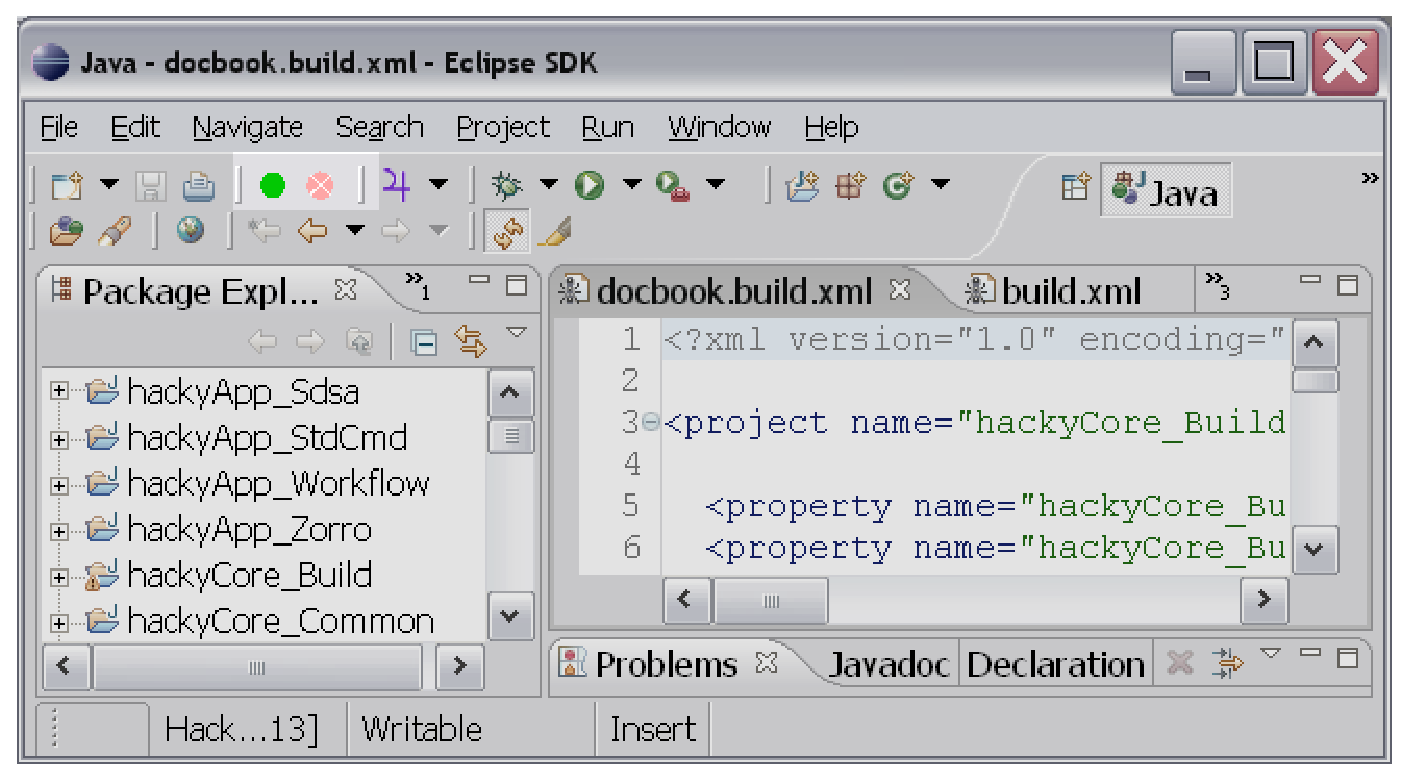
\includegraphics[width=0.6\textwidth]{figs/esr-gui.eps}
  \caption{ESR user interface}\label{fig:esr-gui}
\end{figure} 
\begin{figure}[htbp] 
  \centering
  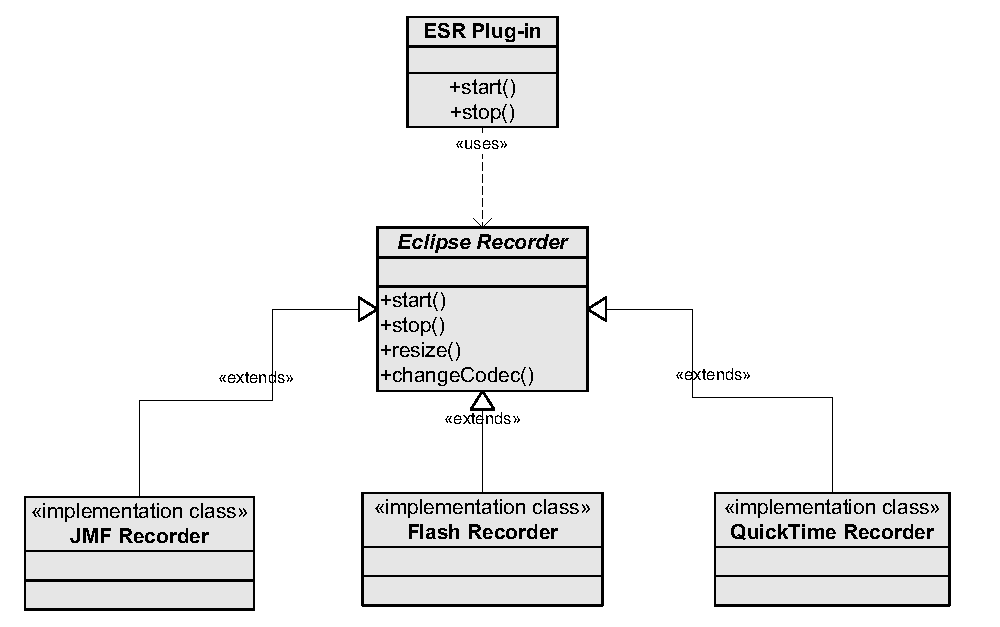
\includegraphics[width=0.9\textwidth]{figs/esr-structure.eps}
  \caption{ESR Plug-in Structure}\label{fig:esr-plugin}
\end{figure} 
interface, which consists of a green button and a red button only in
Eclipse toolbar menu. Internally, ESR defines one abstract recorder and
three concrete recorder implementations using Java Media Framework, Flash
and Quick Time respectively as shown in figure \ref{fig:esr-plugin}.

\subsection{Using ESR}
We recommend QuickTime recorder because its video compressing rate is the
highest one among three ESR recorders: the size of one hour's software
development movie file typically ranges 5mb-10mb depending on main frame
changes and resolution preference. The only down side is that a fast
computer is desired for QuickTime recorder functioning well without causing
noticeable delay of response to software development activities in Eclipse
IDE.

ESR can be easily configured using Eclipse preference page as shown in
figure \ref{fig:esr-preference}.
\begin{figure}[htbp] 
  \centering
  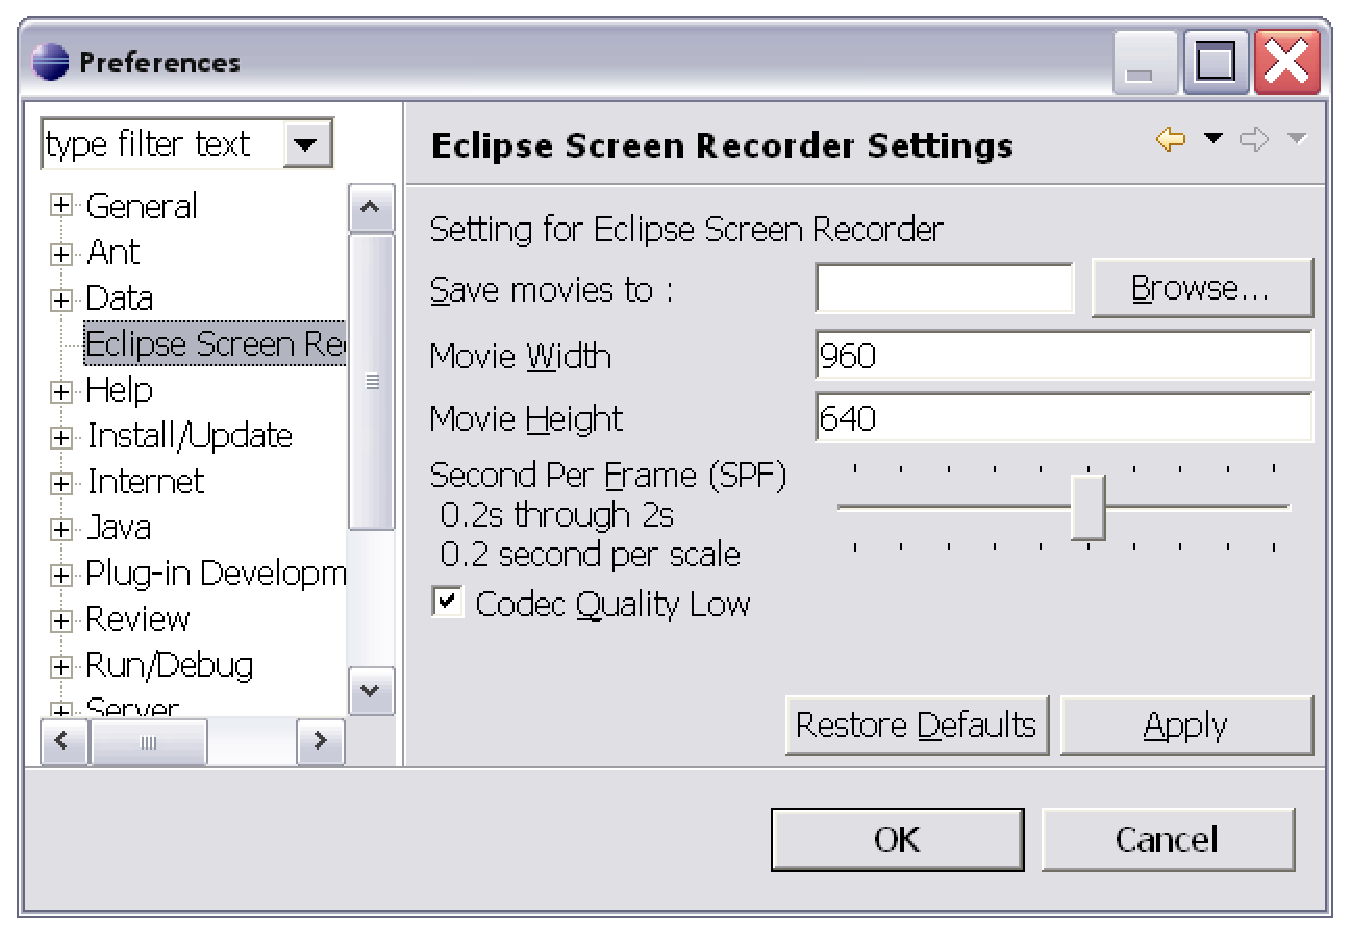
\includegraphics[width=0.8\textwidth]{figs/esr-preference.eps}
  \caption{Configuration of ESR Plug-in}\label{fig:esr-preference}
\end{figure} 
Practical use of ESR found that it can capture 1280*1024 Eclipse window in
one frame per second rate, resize it to 960*680 image and create QuickTime
movie without significant lagging on a 2GHz PC.

\section{Pilot study}
\label{sec:pilot}
\subsection{Subjects}
\subsection{Experiment setting}
\subsection{Procedure}
\subsection{Data analysis}
\subsection{conclusion and discussion}

\section{Classroom study}
\label{sec:classroom}
The pilot study (Section \ref{sec:pilot}) proves that Zorro can collect
enough developer behavior data to derive test-driven development in high
accuracy, in the mean time it also confirms us that the validation study
procedure works well. To be statistically correct, we will conduct an
extended replication Zorro validation study in a software engineering class
in fall 2006.

\subsection{Goals and hypotheses}
As an extended study of pilot study on Zorro validation, the goal of this
study is to validate Zorro's capabilities on developer behavior data
collection and test-driven development recognition. Hypotheses to test are:
\begin{itemize}
\item{Hypothesis 1. }\textit{Zorro can collect enough developer behavior
    data to recognize test-driven development.}
\item{Hypothesis 2. }\textit{Zorro can correctly infer test-driven
    development with the collected developer behavior data.}
\item{Hypothesis 3. }\textit{Zorro can detect alternative processes when
    developers do not do test-driven development.}
\end{itemize}

Kent Beck, pioneer of test-driven development, ever claimed that developers
would be ``test infected'' after they give it a serious try. With the
capability of this study, we will evaluate this claim as well. The fouth
hypothesis is:
\begin{itemize}
\item {Hypothesis 4. } \textit{Students will get ``test infected'' and
    stick to tdd in their course projects development although test-driven
    development is elective.}
\end{itemize}

\subsection{Subjects}
Test subjects are students in a graduate level software engineering class.
Prior to the study we will ask students to sign consent form (see appendix
\ref{app:consent}) to inform them that this study is part of a scientific
research, data collected will not be used against their gradings and
participation is voluntary.  Human subject clearence exemption of this
reseach project was already granted by University of Hawaii Committee on
Human Studies.

\subsection{Experiment setting}
Elements of Zorro validation are Zorro-compliant IDE, Hackystat sensor for
developer behavior collection and ESR for development process recording.
Currently, only Eclipse IDE has a sensor that is designed to collect
development events suitable for Zorro processing. Hackystat Eclipse sensor
and ESR will be used to instrument students' test-driven development
process for colleting development data. In a nutshell, required experiment
settings are:
\begin{itemize}
\item \textit{Windows-based pc(\begin{math}\ge\end{math}1.8GHz CPU and
    \begin{math}\ge\end{math}512MB RAM})
\item \textit{JDK 1.4 or JDK 5}
\item \textit{Eclipse SDK 3.2}
\item \textit{Hackystat Eclipse Sensor (up-to-date version)}
\item \textit{ESR with QuickTime(up-to-date version)}
\end{itemize}

As discussioned in section \ref{sec:esr}, this experiment will not be
conducted in laboratory setting which may deflect how students write
program in actual situation. Instead, student participants will work on
their own PCs at the time to their conveniences.

\subsection{Experiment procedure}
Experiment procedure of this study includes four steps --- training,
practice of test-driven development, enactment of test-driven development,
and course project development in elective process.

\subsubsection{Training}
Software testing is a major topic of software engineering, but it used to
be taught by instructors in a later time as a software quality assurance
technique following the waterfall model. Modern software development
intends to emphasize on software testing at early stage of software process
to improve software quality. Thus, lectures on software testing will be
given at an early time in the software engineering class. Recommended
lectures are:
\begin{itemize}
\item {Lecture 1.} \textit{Software testing methods: system testing,
    validation testing, integration testing and unit testing. Reading
    materials: software testing chapter of textbook.}
\item {Lecture 2.} \textit{Methods and tools: xUnit, JUnit, JUnit in
    Eclipse, JUnit for ANT and Test-Driven Development. Reading materials:
    JUnit 3.8 Cookbook, preface and chapters 1-2 of book ``Test-Driven
    Development by Example''\cite{Beck:03}.}
\item {Lecture 3.} \textit{Software metrics, Hackystat infrastructure,
    software project telemetry. Assignment: install Hackystat sensor,
    develop some simple code, and invoke Hackystat analyses.}
\item {Lecture 4.} \textit{Test-Driven Development, Zorro software system,
    and Eclipse Screen Recorder. Assignment: install and configure ESR,
    develop a trivial problem in TDD with Eclipse sensor and ESR
    instrumentation.}
\end{itemize}

Consent form (appendix \ref{app:consent}) will be distributed to students
after we make sure that students can get along well with Hackystat and ESR.

\subsubsection{Practice of test-driven development}
It is needed and necessary to practice test-driven development for students
from a lesson learned in the pilot study: although test subjects were
explicitly told to do test-driven development with the supplied task list,
50\% episodes are neither test-driven nor refactoring in pilot study. In
addition, it is important to ensure that students are comfortable with
JUnit, test-driven development and instrumentation tools --- Eclipse sensor
and ESR. Therefore, we will ask students to practice test-driven
development on a well-known problem with the supplied tutorial chosen from
the following three candidates:
\begin{itemize}
\item Roman numeral converter: \textit{is a program that can convert any
    integer number between 1 and 50 to roman numeral.}
\item Stack: \textit{is a data structure that works in Last-In-First-Out
    principle.}
\item Bowling game: \textit{a single bowling game consists of ten frames.
    In each frame the object is to roll a ball at ten bowling pins.}
\end{itemize}

The practice of test-driven development will be instrumented by Hackystat
Eclipse sensor and ESR, and the collected data will be used to validate
Zorro. With this practice we will know that:
\begin{itemize}
\item \textit{students understand red/green/refactor rhythm of TDD with
    hands-on experience;}
\item \textit{students can get along well with ESR, the screen recording
    tool.}
\end{itemize}

A follow-up survey (see appendix \ref{app:pre-survey}) will be given to
students to investigate their opinions on test-driven development after
they finish the test-driven development assignment.

\subsubsection{Enactment of test-driven development}
In the previous step, students practice test-driven development on a well
defined problem with step-wise tutorial, which might be too easy compared
to actual problems in software development. Therefore, we will ask students
to work on their course projects using test-driven development for a while.
Purpose of this study is to: validate Zorro with actual software
development data; and urge students do test-driven development seriously.

Same as last step, students will develop software in Eclipse IDE with the
instrumentations of Hackystat Eclipse sensor and ESR. It required to do
more than 3 hours' test-driven development in the first week after course
projects are assigned. Development activity data and ESR video are
collected for Zorro validation analysis.

Another survey (apprendix \ref{app:post-survey}) will be conducted
thereafter to readdress student's opinions on test-driven development and
intention to continue using it in their future software development.

\subsubsection{Course project development in elective process}
In the rest of course project, we will no longer ask student to do
test-driven development and record development process with ESR. In turn,
students can choose any development method that works best for them and
their development process will be instrumented by Eclipse sensor only.

\subsection{Data analysis}
\subsubsection{Test-Driven Development recognition with Zorro}
Hackystat Eclipse sensor collects development activity data and send them
to Hackystat server automatically. A Hackystat project can be defined for
each student to recognize test-driven development with collected
development event data. Figure \ref{fig:zorro-gui} demonstrates Zorro
recognition results for project ``StackWithTDD''.
\begin{figure}[htbp]
  \centering
  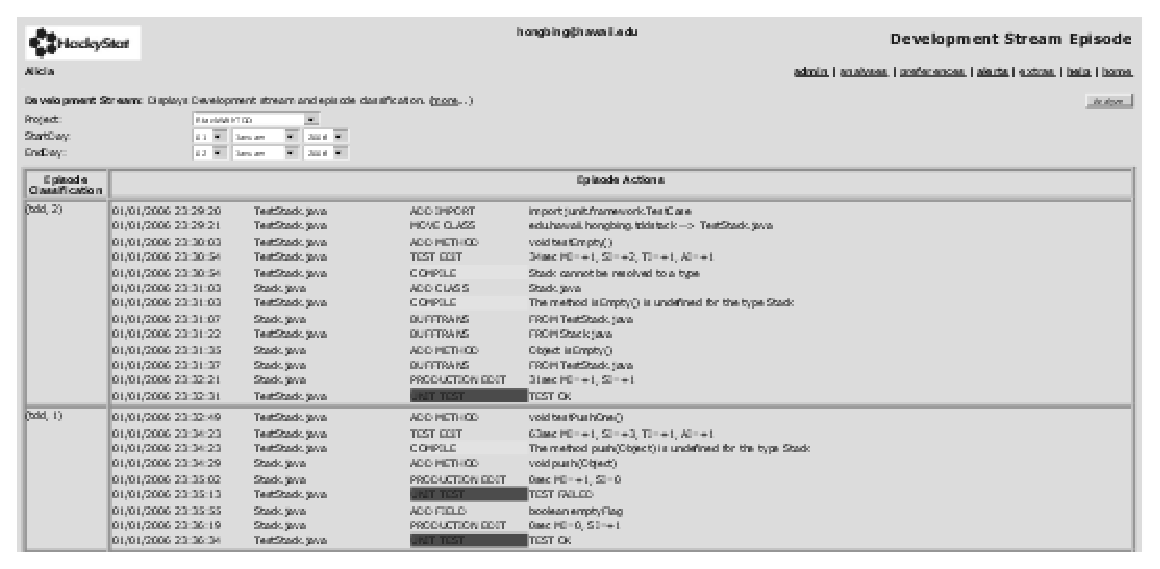
\includegraphics[width=0.85\textwidth]{figs/zorro-interface.eps}
  \caption{Zorro Recognition Results}\label{fig:zorro-gui}
\end{figure} 
Zorro divides the software development stream into episodes and reports the
recognition results of episodes on left column in values---``tdd'',
``tld'', ``refactor'', or ``validation''. Developer behavior data drived
from development events and metrics for test-driven development inference
are displayed on the right column. Each activity includes timestamp when
the activity occurs, file that it is associated with, activity type, and
supplemental metric data.

\subsubsection{Development process video analysis}
In the development process video analysis, we will play the collected
videos with QuickTime player, write down the script of the development
process with a book keeping tool such as Microsoft Excel, and compare them
against development event data collected by Zorro for validation. Figure
\ref{fig:esr-video} is a screen copy of the
\begin{figure}[htbp]
  \centering
  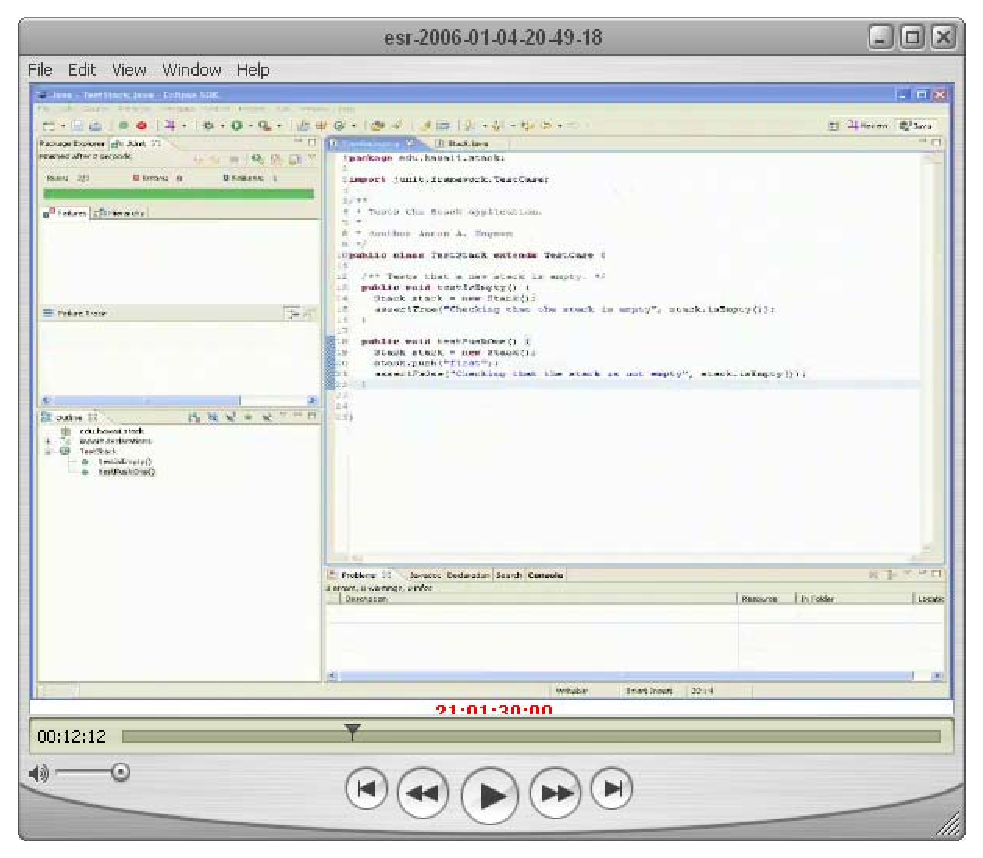
\includegraphics[width=0.8\textwidth]{figs/esr-video.eps}
  \caption{Video of Development Process}\label{fig:esr-video}
\end{figure} 
development movies. The main screen is Eclipse window which records
development activities, and a time line track is attached to the movie at
the bottom for data synchronization. Table \ref{tab:video-narrate}
illustrates how we use Excel to do book keeping and Zorro validation.
\begin{table}[htbp]
\centering
  \caption{Zorro and ESR video comparison data sheet}\label{tab:video-narrate}
  \begin{tabular}{|l|l||l|l|l|l|p{3.5cm}|} \hline 
    \multicolumn{3}{|l}{Subject id: XXX-XX-XXX} & \multicolumn{4}{l|}{Movie file: esr-YYYY-mm-DD-hh-mm-ss.mov} \\ \hline\hline
    Episode \# & Zorro & Video & From & To & Activity & Annotation \\ \hline
    1 & (tdd, 1) & (tdd, 1) & 23:28:32 & 23:28:43 & New project & Create new project HelloWorld \\ \hline
          &          &          & 23:28:45 & 23:29:21 & New TestStack & Create unit test TestHello in package edu.hawaii.ics.rainer \\ \hline
          &          &          & 23:29:55 & 23:30:08 & Add testAloha & Add a empty test case for Hello \\ \hline
          &          &          & ...      & ...      & ... & ... \\\hline
          &          &          & 23:32:26 & 23:32:32 & Run TestHello & Test passes \\ \hline\hline
    2 & (tdd, 1) & (tld, 1) & ... & ... & ... & ... \\ \hline
          &          &          & ... & ... & ... & ... \\ \hline
  \end{tabular}

\end{table}
One by one comparison between bookkeeping data and Zorro developer behavior
data will give us insights whether Zorro data collection mechanism is
correct and whether the collected data are good enough to infer test-driven
development. A beauty of the video analysis is that it can give us insights
how software process is executed by developers, with which we can not only
validate Zorro but also find ways to improve it.

\subsubsection{``Test infected'' claim verification with telemetry}
Software telemetry \cite{csdl2-04-11} is a new approach of software project
management and telemetry report can give retrospective and in-process
analysis on software development process. Zorro defines three telemetry
reduction functions:
\begin{itemize}
\item \textit{MemberTestDriven} Computes Test-Driven Development percentage
  of a project member over the given time interval.
\item \textit{ProjectTestDriven} Computes Test-Driven Development
  percentage of a project over the given time interval.
\item \textit{ZorroEpisode} Reports number of episodes of a specific
  episode type, or total number of test-pass episodes over the given time
  interval.
\end{itemize}

By combining telemetry reports and students survey, we can verify whether
students get ``test-infected'' with strong evidences.

\subsection{Anticipated Results}
\begin{itemize}
\item Zorro collects development necessary behavior data correctly to
  derive test-driven development.
\item Zorro recognizes test-driven development in acceptable accuracy.
\item Students get ``test-infected'' and they continue using test-driven
  after Zorro validation study.
\end{itemize}

\section{Study in TDD community}
\label{sec:community}
Case study with students in classroom setting is insufficient for
generalization of conclusions as the matter of fact that students are
novice programmers and TDD developers. I plan to conduct an off-site case
study of Zorro by recruiting experienced TDD developers from test-driven
development community, the user group of TDD.

\subsection{Goals and hypotheses}
The objective of this study is to validate Zorro on developer behavior data
collection and test-driven development process recognition with experienced
TDD developers. Beyond this objective, I also aim at improving test-driven
development recognition capability of Zorro in actual software development
process. Propositions with regard to these goals are:
\begin{itemize}
\item{Hypothesis 1. }\textit{Zorro can collect enough developer behavior
    data to recognize test-driven development.}
\item{Hypothesis 2. }\textit{Zorro can correctly infer test-driven
    development with the collected developer behavior data.}
\item{Hypothesis 3. }\textit{Zorro helps experienced tdd developers stay on
    the track of test-driven development.}
\end{itemize}

\subsection{Subjects}
Test subjects are experienced TDD developers from the community of
test-driven development, user group of \cite{TddYahooGroup}. On the
account that I only have limited experience on recruiting
experienced/professional developers as test subjects, it will be wise to
take Benestad's advice \cite{Benestad}:
\begin{quote}
  first, practical constraints must be defined when defining the target
  population of software developers; second, participants must be offered
  flexibility and value using a planned communication strategy; third, high
  professional and ethical standard must be employed.
\end{quote} 
There principles are largely for recruiting professional developers from
software organizations for controlled experiments, but we can borrow the
idea to assist recruiting test-driven development community members who
likely belong to some software institutes.

\begin{enumerate}
\item \textit{Practical constraint must be defined when defining the
    target population of software developers.}\\
  The constraint is that participants must be okay with Java programming in
  Eclipse IDE in Windows OS. JUnit 3.8 is recommended.
\item \textit{Participants must be offered flexibility and value.}\\
  Test subjects have the flexibility to choose the problem to tackle in
  test-driven development to their conveniences. Process Instrumentation
  and data collection overhead are maintained in the lowest level. As the
  payback, participants can use Zorro in their organizations for
  test-driven development process improvement and I will provide technique
  support. Appendix \ref{app:letter} is the participation solicitation
  letter for recruiting experienced developers from test-driven development
  community.
\item \textit{High professional and ethical standard must be employed.}\\
  Clearence of human subject exemption was already granted by University of
  Hawaii Committee on Human Studies. Participants' individual skills will
  not be evaluated, instead their inputs will be used to evaluated Zorro
  software system. The participantion of this study is voluntary and test
  subjects can withdraw from the study at any time. A consent form
  (appendix \ref{app:consent2}) will be signed by participants and they can
  keep a copy of it for reference.
\end{enumerate}

\subsection{Experiment setting}
This study offers the flexibility to allow participants work off-site at
their own working environment. Basic requirements are:
\begin{itemize}
\item \textit{Windows-based pc(\begin{math}\ge\end{math}1.8GHz CPU and
    \begin{math}\ge\end{math}512MB RAM})
\item \textit{JDK 1.4 or above}
\item \textit{Eclipse}
\item \textit{JUnit 3.8}
\item \textit{Hackystat Eclipse Sensor}
\item \textit{Eclipse Screen Recorder}
\item \textit{Quick Time}
\end{itemize}
Java 5 features of JUnit 4.x are depressed for this study because Eclipse
sensor can not tell on-going metrics of Java 5 style code. In order to help
participants configure the test environment, we wrote a DocBook chapter for
reference in HTML at \cite{ZorroUserGuide}.

\subsection{Data collection}
The Java development in Eclipse IDE in test-driven development will be
instrumented by Hackystat Eclipse IDE and ESR. Once installed, Hackystat
Eclipse sensor can collect data unobtrusively. Developers start ESR
recording by pressing green button and stop it by pressing red button.
It takes test subject's manual intervention to send the recorded movie file
to reseachers for data analysis.

\subsection{Procedure}
\subsubsection{Recruition of test subjects}
A participation invitation email will be sent to test-driven development
user group to recruit test subjects. The first contact email will briefly
address objective of this study, introduction of Zorro software system and
what participants will do in the study. If some people are interested in
participation, I will send them consent form and instruction guideline for
the study.

\subsubsection{Test environment setup}
Participants will install Eclipse IDE if they've not done it yet, and
process instrumentation utilities --- Hackystat Eclipse sensor and Eclipse
screen recorder (ESR) under help of Zorro user guide\cite{ZorroUserGuide}.

\subsubsection{Development and data collection}
Developers can choose the problem they want to work on either from the
selected problem sets or elect their own software development in TDD.
\begin{itemize}
\item A well-known problem: stack, roman numeral or bowling game.
\item Another interested problem: money, sudoku, or spreadsheet.
\item 1-3 hours' personal software development in TDD.
\end{itemize}
The development process is instrumented by Hackystat Eclipse sensor and ESR
for data collections. Developers will send their recorded process video to
me using email for data analysis and answers to a short survey on usfulness
and usability of Zorro software system.

\subsection{Data analysis}
\subsubsection{Zorro validation analysis} 
We will be conducting similar analysis as in classroom case study
\ref{sec:classroom} to validate Zorro's data collection and TDD recognition
capability.

\subsubsection{Usefulness and usability of Zorro}
Feedback from experienced TDD developers is helpful on identifying issues
regarding to test-driven development discipline in practice and verifying
hypothesis 3 made on Zorro usefulness.




